\section{Prospettive sulla programmazione parallela}
Uno degli aspetti più importanti della programmazione parallela, è analizzare il problema e capire se può essere parallelizzato. La parallelizzazione del codice porta a dei miglioramenti delle performance solo se il workload (peso computazionale) è non trascurabile.
Seguono alcune definizioni
\begin{itemize}
    \item \textbf{Task: } unità di esecuzione o di lavoro di un programma o di un sottoprogramma. Le istruzioni sono eseguite sequenzialmente ovvero non in parallelo.

    \item Processo/thread: entità astratta che esegue i task assegnati ai processi. I processi comunicano tra di loro e si sincronizzano per eseguire i loro task.
    \item Processore: motore fisico su cui ciascun processo viene eseguito. Il programma viene scritto come un insieme di processi che vengono poi mappati sul processore.
\end{itemize}

\subsection{Step per creare un programma parallelo}
\begin{figure}[th]
	\centering
	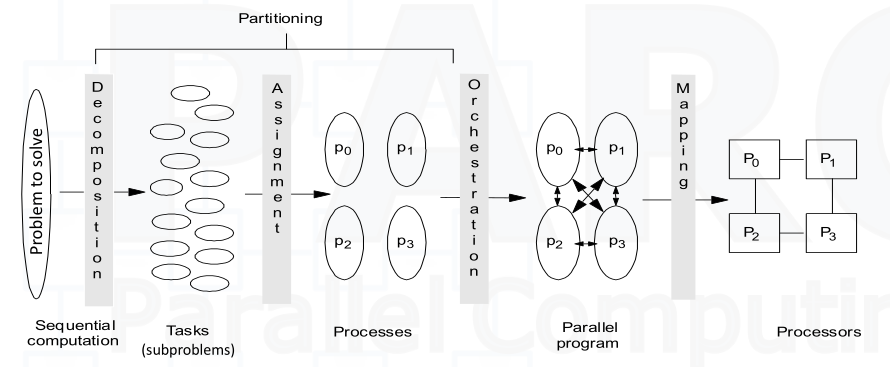
\includegraphics[width=0.7\linewidth]{img/4-step-programma-parallelo}
	\caption{i 4 step per creare un programma parallelo.}
	\label{fig:4-step-programma-parallelo}
\end{figure}

Ci sono 4 passi nella creazione di un programma parallelo:
\begin{enumerate}
    \item Decomposizione dell'algoritmo risolutivo in task o sottoproblemi;
    \item Si assegnano le varie task ai processi; 
    \item Orchestrazione dell'accesso ai dati, comunicazione e sincronizzazione  da parte dei processi;
    \item Mapping dei processi ai processori ()un processo non può essere assegnato a più unità di calcolo).
\end{enumerate}

Il livello di parallelismo viene determinato nelle fasi di decomposizione e assegnamento.

\subsubsection{Comprensione del problema/programma}
Indubbiamente, il primo passo nello sviluppo di software parallelo è capire innanzitutto il problema che si desidera risolvere in parallelo. Se si parte da un programma seriale, ciò implica anche la comprensione del codice esistente.

Prima di investire tempo nel tentativo di sviluppare una soluzione parallela per un problema, bisogna determinare se il problema può effettivamente essere parallelizzato.


\begin{enumerate}
    \item Identificare gli \textbf{hotspot} del programma: rappresentano le parti dove viene svolta la maggior parte del lavoro effettivo. La maggior parte dei programmi scientifici e tecnici di solito svolgono la maggior parte del loro lavoro in pochi punti. Gli strumenti di profilazione e analisi delle prestazioni possono aiutare ad individuare gli hotspote .profiling\footnote{I tool di profiling eseguono il codice e, assieme al suo risultato, ritornano anche un report che può contenere: il numero di invocazioni per ogni funzione contenuta nel codice, e il tempo che impiega ciascuna per determinare il risultato che calcola, quali sono le parti del codice più usate, e così via,\dots} e analisi delle performance (tramite appositi tool). Gli hotspot sono generalmente le sezioni in cui si concentra la parallelizzazione e che hanno un utilizzo della CPU alto.
    \item Identificare i \textbf{bottleneck} del programma: sono le aree di codice che sono più lente da eseguire (come ad esempio le sezioni dedicate all'I/O). Una possibile strada che si può seguire per contrastare i bottleneck, consiste nel trasferire la loro esecuzione sulla GPU, in modo da non dover rallentare la CPU. Dunque, si possono vedere due livelli di parallelismo: il primo dato dalla parallelizzazione su GPU del codice, mentre il secondo dato dalla concorrenza di esecuzione di CPU e GPU.
    \item Identificare gli\textbf{ inibitori al parallelismo}: analizzare il problema significa anche identificare gli inibitori del parallelismo, che sono quei fattori che impediscono di parallelizzare il codice. Una classe comune di inibitori è la dipendenza dei dati, come dimostrato dalla sequenza di Fibonacci sotto.
\end{enumerate}

\underline{Esempio di problema parallelizzabile}: Calcolare l'energia potenziale per migliaia di diverse conformazioni molecolari indipendenti. Una volta completato, individua la conformazione molecolare con l'energia potenziale minima. Ogni conformazione molecolare è determinabile in modo indipendente e il calcolo dell'energia potenziale minima è parallelizzabile.
\\

\underline{Esempio di problema non-parallelizzabile}: Calcolare la serie di Fibonacci. Questo problema non è parallelizzabile in quanto il calcolo attuale dipende dai calcoli precedenti (il termine $k+2$ è dato dalla somma dei termini $k+1$ e $k$). 
\\



\subsubsection{Decomposizione}
Nella decomposizione (o scomposizione) di un problema in task, è cruciale individuarne un numero appropriato in modo che ci siano sempre thread sufficienti per mantenere i processori occupati. In una configurazione con 100 processori funzionanti in parallelo, è necessario avere un ampio pool di task per garantire che tutti i processori siano costantemente utilizzati, anche se uno dei compiti si blocca. È comune che un task raggiunga un punto in cui necessita di dati da un altro task o deve eseguire operazioni di I/O, interrompendo temporaneamente l'esecuzione e lasciando il processore inutilizzato. L'obiettivo è minimizzare questa inattività, assicurando che un nuovo task sia pronto per essere eseguito non appena un processore si libera. Ogni core o processore lasciato inattivo rappresenta uno spreco di risorse. Pertanto, è essenziale disporre di un numero sufficiente di task prontamente disponibili per sostituire quelli bloccati e massimizzare l'utilizzo dei processori.

Esistono due modi per scomporre in task:
\begin{itemize}
    \item \textbf{Scomposizione di dominio:} il dominio può essere suddiviso tra le istanze del task in diverse modalità a seconda delle dimensioni del problema (figura \ref{fig:domain-decomposition}). Ad esempio, se si considera la somma di tutti i dati di un array, questa operazione può essere suddivisa a livello di blocchi o a livello ciclico (figura \ref{fig:slicing-techniques}). Nel primo caso, i dati sono divisi in blocchi distinti assegnati a diverse istanze per l'elaborazione. Nel secondo caso, ogni istanza elabora sequenzialmente una cella di memoria dopo l'altra, seguendo un ciclo, e le celle sono divise da una distanza. 
        \begin{figure}[th]
    	\centering
    	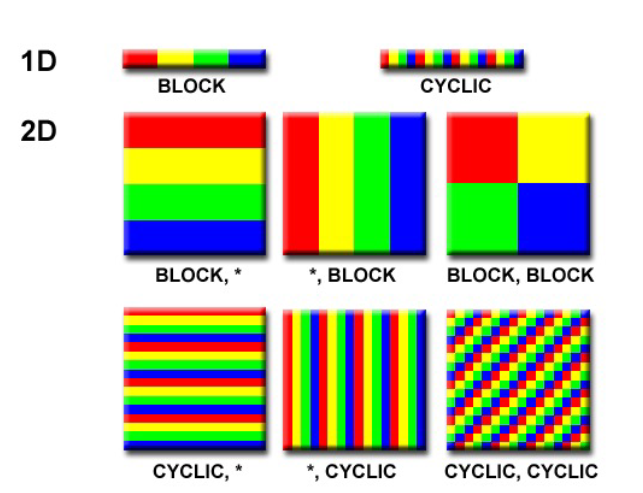
\includegraphics[width=0.7\linewidth]{img/domain-decomposition.png}
    	\caption{scomposizione di dominio.}
    	\label{fig:domain-decomposition}
    \end{figure}
    
    Anche nel caso di domini a due dimensioni, come le matrici, è possibile suddividere l'elaborazione in vari modi. Si possono suddividere i dati in blocchi orizzontali, verticali o a mattonelle. Altrimenti, l'elaborazione può essere ciclica nelle righe, nelle colonne o negli elementi della matrice. Un fattore importante da tenere presente è il bilanciamento del carico (\textbf{load balancing}). se siamo sicuri che il tempo impiegato dalla prima thread sul blocco A corrisponde a quello impiegato dalla seconda thread sul blocco B e così via per il resto dei blocchi, allora abbiamo un carico bilanciato. Questo di solito è il caso per problemi lineari. Quando però abbiamo problemi più complessi, il carico di lavoro di una thread diventa imprevedibile. In questo caso potrebbe essere più ottimale aumentare i blocchi facendo in modo che il primo processore che si libera vada a prendere la successiva thread in attesa.
    \begin{figure}[th]
    	\centering
    	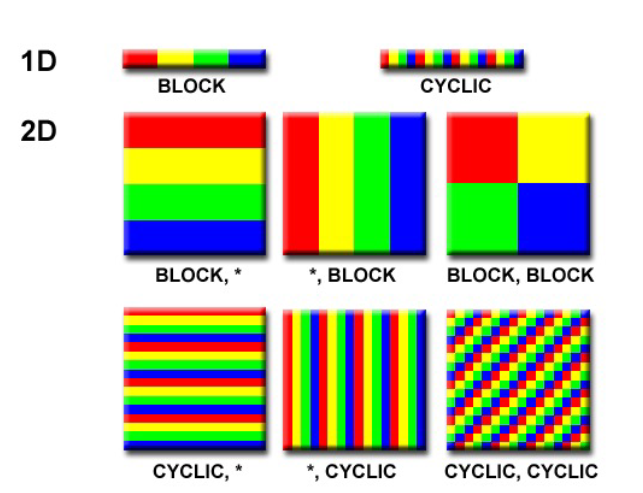
\includegraphics[width=0.7\linewidth]{img/slicing-techniques.png}
    	\caption{i vari modi in cui un dominio può essere scomposto.}
    	\label{fig:slicing-techniques}
    \end{figure}

    \item \textbf{Scomposizione funzionale:} ci si concentra sull'elaborazione che deve essere fatta piuttosto che sui dati manipolati dalla computazione. Il problema è quindi scomposto rispetto al lavoro che deve essere fatto. Ogni task esegue parte del lavoro totale (figura \ref{fig:functional-decomposition}).
        \begin{figure}[th]
    	\centering
    	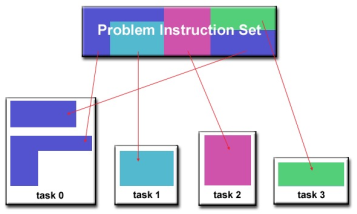
\includegraphics[width=0.7\linewidth]{img/functional-decomposition.png}
    	\caption{scomposizione funzionale.}
    	\label{fig:functional-decomposition}
    \end{figure}
\end{itemize}

La scomposizione è compito del programmatore, che può essere supportato da tool automatici (campo di ricerca).

\subsubsection*{Esempio di parallelizzazione}
Data un'immagine $N\times N$ vogliamo:
\begin{enumerate}[label=$\bullet$ \textbf{Step \arabic*:}]
    \item raddoppiare la luminosità di ogni pixel; {\color{NavyBlue}\textbf{(complessità $N^2$)}}
    \item calcolare la media di tutti i pixel. {\color{NavyBlue}\textbf{(complessità $N^2$)}}
\end{enumerate}

\paragraph{Soluzione sequenziale.} Una soluzione sequenziale di questo problema costa un tempo totale di {\color{NavyBlue}$N^2+N^2=2N^2$} (figura \ref{fig:esecuzione-sequenziale}). 
\begin{figure}[th]
	\centering
	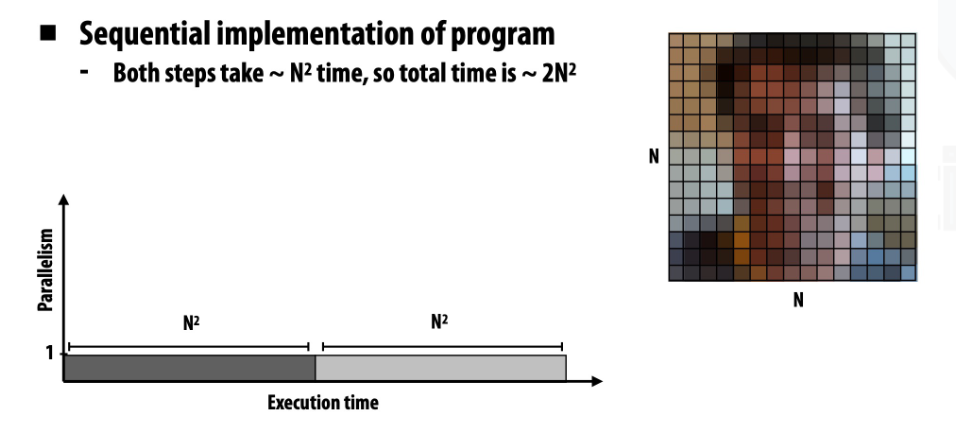
\includegraphics[width=0.7\linewidth]{img/esecuzione-sequenziale.png}
	\caption{Esecuzione sequenziale.}
	\label{fig:esecuzione-sequenziale}
\end{figure}

\paragraph{Parallelizzazione sulla prima fase.}Una strategia di parallelizzazione consiste nell'eseguire in parallelo lo step 1, completandolo in $\frac{N^2}{P}$ (figure \ref{fig:esecuzione-parallela-1}), dove $P$ rappresenta il numero di processori disponibili. Invece parallelizzare lo step 2 risulta inefficiente  per via della interdipendenza tra i pixel dell'immagine nell'applicazione del filtro, dunque il suo costo è di $N^2$. Lo speedup stimato risulta:
\begin{align*}
    speedup &\le \frac{2N^2}{\frac{N^2}{P} + N^2}\\
    &\le 2
\end{align*}

\begin{figure}[th]
	\centering
	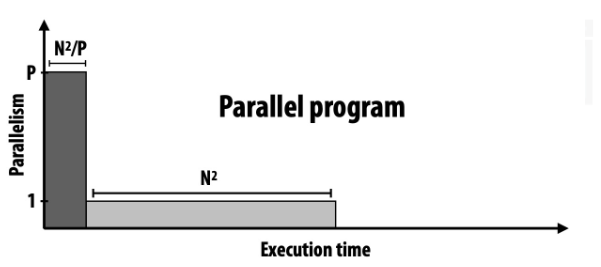
\includegraphics[width=0.7\linewidth]{img/esecuzione-parallela-1.png}
	\caption{Primo tentativo di parallelismo.}
	\label{fig:esecuzione-parallela-1}
\end{figure}

\paragraph{Parallelizzazione sulla seconda fase}Un miglioramento potrebbe essere ottenuto parallelizzando il calcolo della media su ${P}$ processori (calcolo su $P$ matrici di dimensione $\frac{ N^2}{P}$ -- figura \ref{fig:esecuzione-parallela-2}). Infine viene introdotto un tempo di overhead dovuto alla combinazione delle somme parallele per ottenere il risultato finale. I tempi diventano:
\begin{align*}
    \text{Tempo step 1 } &= \frac{N^2}{P}\\
    \text{Tempo step 2 } &= \frac{N^2}{P}+P    
\end{align*}

e si ottiene uno speedup pari a:
\begin{align*}
    speedup \le \frac{2N^2}{\frac{2N^2}{P} + P}\\
\end{align*}

\begin{figure}[th]
	\centering
	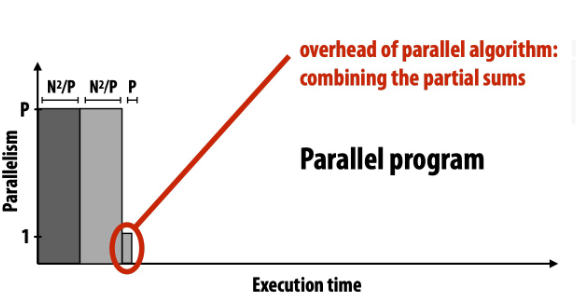
\includegraphics[width=0.7\linewidth]{img/esecuzione-parallela-2.png}
	\caption{Secondo tentativo di parallelismo.}
	\label{fig:esecuzione-parallela-2}
\end{figure}

\subsubsection{Assegnamento}
Questo processo richiede la creazione di un numero adeguato di task e la loro distribuzione tra i processi disponibili.

Per prima cosa, è necessario determinare quanti processi sono necessari e quindi associare i task ai processi. Tipicamente, il numero di processi è uguale al numero di processori disponibili per garantire una concorrenza massima.

La strategia di assegnazione dipende dall'esperienza e dalla conoscenza del problema. È consigliabile raggruppare task che richiedono comunicazione tra loro nello stesso processo per accelerare la comunicazione. Al contrario, task che possono eseguire indipendentemente possono essere distribuiti tra processi diversi per ridurre il carico su ciascun processore.

Tuttavia, è cruciale considerare il bilanciamento del carico (\textbf{load balancing}) durante l'assegnazione dei task. Un'assegnazione sbilanciata può compromettere le prestazioni del sistema anche se il codice è parallelizzato correttamente. Ad esempio, se alcuni processi ricevono task più pesanti di altri, potrebbero diventare il collo di bottiglia del sistema, rallentando l'intera esecuzione.

Il tempo di esecuzione complessivo del codice è determinato dal tempo impiegato dal processo più lento, non dalla media dei tempi di esecuzione. Di conseguenza, è fondamentale evitare sbilanciamenti nella distribuzione dei task per massimizzare l'utilizzo dei processori disponibili.

Il miglioramento dell'assegnamento dei task può ridurre gli sprechi di risorse e migliorare le prestazioni complessive del sistema. Anche se non è possibile ottenere un equilibrio perfetto, è importante ridurre al minimo gli sbilanciamenti per sfruttare al meglio le risorse disponibili. Questa ottimizzazione richiede una buona capacità di programmazione e una solida comprensione del problema e dell'architettura del sistema.


\begin{figure}[th]
	\centering
	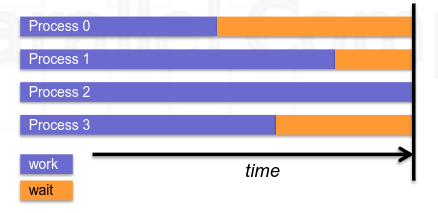
\includegraphics[width=0.7\linewidth]{img/barrier-sync.png}
	\caption{Esempi di punto di sincronizzazione.}
	\label{fig:barrier-sync}
\end{figure}

Il bilanciamento del carico è cruciale per ottenere prestazioni ottimali in un ambiente di elaborazione parallela, come quello di CUDA. Esistono varie strategie per garantire un bilanciamento efficace del carico di lavoro.

In alcuni casi, è possibile determinare staticamente il peso computazionale di ciascun processo attraverso il profiling e l'analisi delle prestazioni. Tuttavia, ci sono situazioni in cui il peso computazionale dipende dall'input o da altri fattori dinamici, rendendo difficile una determinazione statica. Un esempio di ciò è l'algoritmo di attraversamento del grafo BFS (Breadth-First Search), dove il numero di figli di ciascun nodo può variare notevolmente.

Per gestire questa incertezza, è necessario utilizzare tecniche di bilanciamento dinamico del carico. Queste tecniche consentono di assegnare i task ai processi durante l'esecuzione, in base alle condizioni attuali. Sebbene queste tecniche possano aggiungere un carico computazionale aggiuntivo, sono cruciali per garantire un bilanciamento efficace del carico e massimizzare lo speedup complessivo del sistema.

Durante l'esecuzione, i task vengono inseriti in una coda e assegnati ai processi disponibili. Ogni processo prende un task dalla coda e lo elabora, passando al successivo una volta completato il lavoro. Questo approccio permette di gestire dinamicamente il carico di lavoro e adattarsi alle variazioni nelle prestazioni dei task e dei processi.

Per quanto riguarda la granularità dei task, si parla di task \textbf{coarse-grained} e \textbf{fine-grained}. Questa distinzione si basa sulla quantità di lavoro svolto da ciascun task. I task fine-grained sono piccoli e comprendono poche righe di codice, mentre i task coarse-grained sono più grandi e comprendono una quantità maggiore di codice. La scelta tra task coarse-grained e fine-grained dipende dal problema specifico e dalla necessità di bilanciare il carico di lavoro. I task fine-grained sono più facili da bilanciare e consentono un maggior grado di flessibilità nell'assegnazione dei task ai processi, ma possono introdurre un overhead aggiuntivo a causa delle sincronizzazioni. D'altra parte, i task coarse-grained sono più difficili da bilanciare ma possono ridurre l'overhead di sincronizzazione. La scelta dipende quindi dalle esigenze specifiche del problema e dall'architettura del sistema.
\subsubsection{Orchestrazione}
Il focus principale è comprendere come far comunicare e sincronizzare tutti questi task. Si è già trattato dell'architettura \textit{embarassingly paralle}l, in cui i processi sono completamente indipendenti. In questo scenario, la sincronizzazione non è necessaria: è quasi un'utopia. Tuttavia, quando si rende necessaria la comunicazione, si introduce inevitabilmente un overhead rispetto al codice sequenziale.